\documentclass[margin=5mm]{standalone}
\usepackage[dvipsnames]{xcolor}
\usepackage{pgfplots}
\usepackage{tikz}
\usepackage[tikz]{ocgx2}

\pgfplotsset{compat=1.18}
\begin{document}

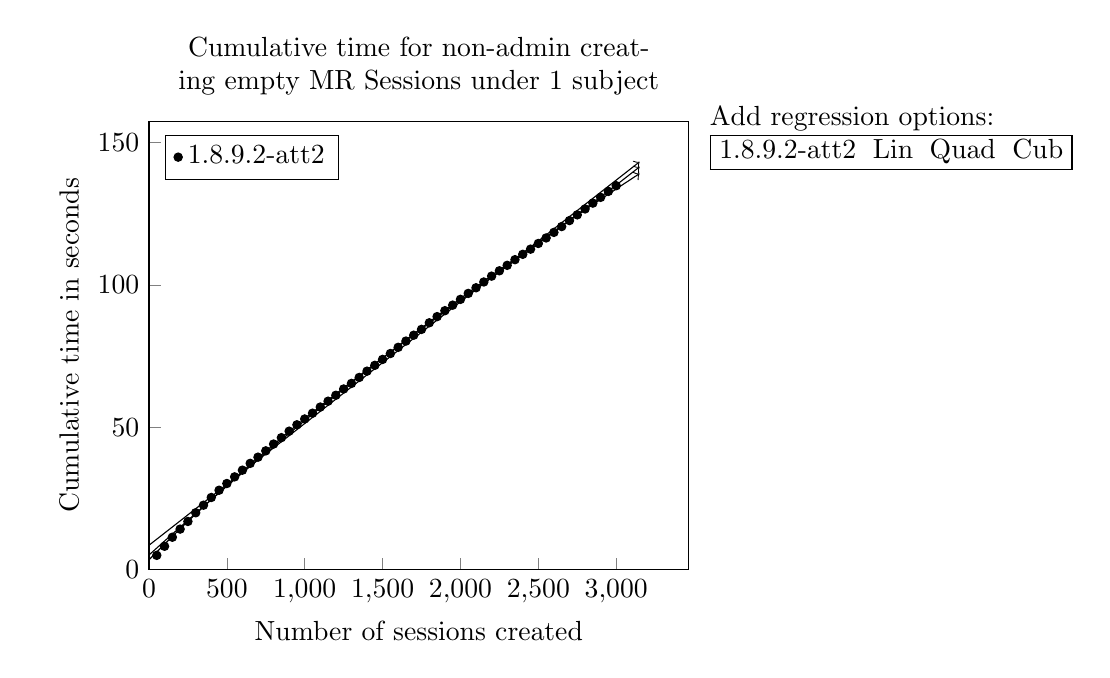
\begin{tikzpicture}
    \begin{axis}[
        align = center,
        legend pos = north west,
        legend cell align = left,
        xlabel = Number of sessions created,
        ylabel = Cumulative time in seconds,
        xtick pos = left,
        ytick pos = left,
        scaled ticks = false,
        xmin = 0,
        ymin = 0,
        title = {Cumulative time for non-admin creating empty MR Sessions under 1 subject},
        title style = {text width = 0.8\textwidth},
        legend entries={\switchocg{1.8.9.2-att2}{1.8.9.2-att2}}]
        \begin{scope}[ocg = {ref = 1.8.9.2-att2-Lin, status = invisible}]
            \plot[domain=0:3150,->,forget plot] (\x,{8.4854796610169440640447646728716790676116943359375 + 0.042773259238677419080687513996963389217853546142578125*(\x)^1});
        \end{scope}
        \begin{scope}[ocg = {ref = 1.8.9.2-att2-Quad, status = invisible}]
            \plot[domain=0:3150,->,forget plot] (\x,{5.04918918760958579383668620721437036991119384765625 + 0.049424144025917472744513503357666195370256900787353515625*(\x)^1 + -0.00000218061796302952584473977548640277746017090976238250732421875*(\x)^2});
        \end{scope}
        \begin{scope}[ocg = {ref = 1.8.9.2-att2-Cub, status = invisible}]
            \plot[domain=0:3150,->,forget plot] (\x,{3.378787693664313085406547543243505060672760009765625 + 0.0557368211229773979908941328176297247409820556640625*(\x)^1 + -0.0000073124197877461779619353600401243653550409362651407718658447265625*(\x)^2 + 0.00000000112170531687795658438474620077589249955707373374025337398052215576171875*(\x)^3});
        \end{scope}
        \begin{scope}[ocg = {ref = 1.8.9.2-att2, status = visible}]
            \addplot[
                only marks,
                color = black,
                mark = *,
                mark size = 1.5 pt
            ]coordinates {(50,4.944)(100,8.13)(150,11.302)(200,14.16)(250,16.851)(300,19.909)(350,22.563)(400,25.274)(450,27.82)(500,30.183)(550,32.524)(600,34.867)(650,37.266)(700,39.44)(750,41.664)(800,44.051)(850,46.292)(900,48.575)(950,50.817)(1000,52.858)(1050,54.885)(1100,57.052)(1150,59.107)(1200,61.197)(1250,63.397)(1300,65.357)(1350,67.452)(1400,69.664)(1450,71.707)(1500,73.796)(1550,75.86)(1600,78.038)(1650,80.237)(1700,82.304)(1750,84.349)(1800,86.668)(1850,88.833)(1900,90.916)(1950,92.859)(2000,94.901)(2050,96.99)(2100,98.972)(2150,101.002)(2200,103.056)(2250,104.938)(2300,106.856)(2350,108.844)(2400,110.722)(2450,112.535)(2500,114.536)(2550,116.471)(2600,118.427)(2650,120.48)(2700,122.578)(2750,124.593)(2800,126.664)(2850,128.717)(2900,130.748)(2950,132.848)(3000,134.836)};
        \end{scope}
    \end{axis}
    \begin{scope}
        \addtolength{\tabcolsep}{-0.3em}
        \node [below right, shape=rectangle, align=left](regressiontable) at (7,6) {
            Add regression options: \\
            \begin{tabular}{|llll|}
                \hline
                1.8.9.2-att2 & \switchocg{1.8.9.2-att2-Lin}{Lin} & \switchocg{1.8.9.2-att2-Quad}{Quad} & \switchocg{1.8.9.2-att2-Cub}{Cub} \\
                \hline
            \end{tabular}
        };
    \end{scope}
\end{tikzpicture}

\end{document}